\section{Experiments over 2 axes}


% Model
Models used for experiments in a 2D environment are just the concatenation of the previous models: 2 double integrator with velocity feedback.
Each of the dynamics over the different axis are decoupled.
The previous results apply for each axis, this being said, we will not talk about the noise.
%Description of the environment, property to verify, LTL stuff and so on.
The environment used to do the tests is described in figure \ref{fig:environment}. We will try to verify the formula $ \varphi = (\LTLalways \neg out) \and (\LTLalways \LTLeventually a) \and (\LTLalways \LTLeventually b)$. 

The size of the models is squared in comparison to the 1D models.
We have been able to find plan solutions for the 1 and 0 input memory extended state abstraction, however the raw abstraction was too complex to find a solution in a decent time.
\comment{size of the fixed points}

\comment{I have to compare the sizes of the abstractions.}

\begin{figure}
	\center
	\includestandalone[width=0.5\textwidth]{2D_env_problem}
	\caption{Testing environment for the quadricopter.}
	\label{fig:environment}
\end{figure}

\comment{Show the simulation, the runs and so on.}

\subsection{$\Ninputs = 1$ input memory model}
See figure \ref{fig:double_reduce_2D}.

\begin{figure*}
	\center
	\includestandalone[width=\textwidth]{double_reduced_2D}
	\caption{$\Ninputs=1$ input memory model in 2D.}
	\label{fig:double_reduce_2D}
\end{figure*}

\subsection{$\Ninputs = 0$ input memory model}
See figure \ref{fig:double_reduce_2D}.

\subsection{Real case scenarios}
See figure \ref{fig:real_case}.
In the case of the wind turbine application, the quad will have to go from the base station to the wind turbine blade and explore a given set of regions while avoiding the blade.
The wind can be modelled as a perturbation on the velocity of the quadricopters.
We have been using the first integrator model in this case.

\begin{figure}[!ht]
  \centering
  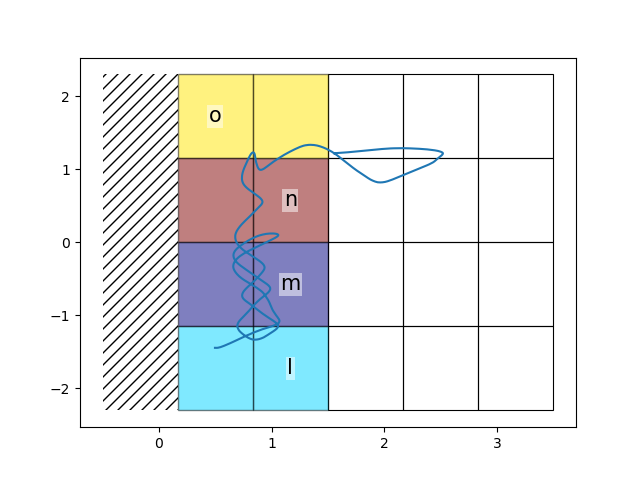
\includegraphics[width=0.9\linewidth]{real_case_scenarios}
  \caption{A trajectory in the state space $(x,v)$.}
  \label{fig:real_case}
\end{figure}

